% Figure: the orbit coordinate and the canonical gauge. Referenced from §6, before
% prop:canonical-gauge. Pure TikZ. Design after the hub's parabolic_grading.py (orbits of
% a scaling action), adapted to a one-dimensional axis.
%
% Pedagogic point, one per panel: (a) on the scale axis as given, S_σ is some increasing
% bijection; the orbit of the point 1, σ ↦ S_σ 1, sweeps the whole axis (no fixed point,
% Lemma 6.2(4)), so the orbit parameter σ can serve as a coordinate. (b) in that
% coordinate, x̃ = χ(x), the same action is multiplication by σ: the axis is straightened.
% The dashed curve is χ itself, drawn as a graph between the two axes.

\begin{figure}[t]
\centering
\begin{tikzpicture}[every node/.style={font=\small}, line cap=round, >=stealth]

% a concrete gauge for the drawing: chi(x) = x^2, so S_σ 1 = sqrt(σ) on the raw axis.
% panel (a) unit 3cm: sqrt(σ) for σ = 1/2, 1, 2, 4 -> 2.12, 3, 4.24, 6
% panel (b) unit 1.5cm: σ itself -> 0.75, 1.5, 3, 6  (σ = 4 lands at the same abscissa)
% ---------- panel (a): the scale axis as given ----------
\begin{scope}[yshift=0cm]
  \node[anchor=west] at (-0.3,1.7) {(a) the scale axis as given: the orbit of $1$ under $\Sact_\sigma$};
  \draw[->] (0,0) -- (8.0,0) node[right] {$x$};
  \draw (0,0.07) -- (0,-0.07); \node[below] at (0,-0.05) {$0$};
  \foreach \p/\l in {2.12/$\Sact_{1/2}1$, 3/$1$, 4.24/$\Sact_{2}1$, 6/$\Sact_{4}1$} {
    \draw (\p,0.07) -- (\p,-0.07); \node[below] at (\p,-0.05) {\l};
  }
  \fill (3,0) circle (1.6pt);
  \draw[->,dashed] (3,0.15) to[bend left=35] node[above] {$\Sact_2$} (4.24,0.15);
  \draw[->,dashed] (4.24,0.15) to[bend left=35] node[above] {$\Sact_2$} (6,0.15);
  \draw[->,dashed] (3,0.15) to[bend right=35] node[above] {$\Sact_{1/2}$} (2.12,0.15);
  \node[anchor=west] at (0,-0.75) {equal ratios of $\sigma$, unequal steps on the axis};
\end{scope}

% ---------- panel (b): the same axis in the canonical gauge ----------
\begin{scope}[yshift=-3.6cm]
  \node[anchor=west] at (-0.3,1.7) {(b) the canonical gauge $\tilde x = \chi(x)$: the same action is multiplication};
  \draw[->] (0,0) -- (8.0,0) node[right] {$\tilde x$};
  \draw (0,0.07) -- (0,-0.07); \node[below] at (0,-0.05) {$0$};
  \foreach \p/\l in {0.75/$\tfrac12$, 1.5/$1$, 3/$2$, 6/$4$} {
    \draw (\p,0.07) -- (\p,-0.07); \node[below] at (\p,-0.05) {\l};
  }
  \fill (1.5,0) circle (1.6pt);
  \draw[->,dashed] (1.5,0.15) to[bend left=35] node[above] {$\times 2$} (3,0.15);
  \draw[->,dashed] (3,0.15) to[bend left=35] node[above] {$\times 2$} (6,0.15);
  \draw[->,dashed] (1.5,0.15) to[bend right=35] node[above] {$\times \tfrac12$} (0.75,0.15);
  \node[anchor=west] at (0,-0.75) {$\chi(\Sact_\sigma x) = \sigma\,\chi(x)$: equal ratios of $\sigma$, equal ratios on the axis};
\end{scope}

\end{tikzpicture}
\caption{The orbit coordinate. (a)~On the scale axis as the family presents it, the action
$\Sact_\sigma$ of (A8) is some increasing bijection; the orbit of the point $1$,
$\sigma \mapsto \Sact_\sigma 1$, is continuous, strictly increasing and has no fixed point, so
it sweeps the whole axis (Lemma~\ref{lem:action-rigidity},
Proposition~\ref{prop:canonical-gauge}). Equal ratios of $\sigma$ are unequal steps on the
axis. (b)~Labelling each point by the $\sigma$ that reaches it, $\tilde x = \chi(x)$, the same
action becomes multiplication by $\sigma$: the canonical gauge. In this gauge every accumulated exponent is a dilate of one function, $G(x,s) = F(\tilde x s)$.}
\label{fig:orbit-gauge}
\end{figure}
